% Thanks http://www.latex-tutorial.com/tutorials/advanced/latex-tikz/
% The package pgf/tikz can be used to create beautiful graphics, especially diagrams in LaTeX. It enables you to create vector graphics from within your document, without the need of external tools such as Inkscape or Adobe Illustrator and thus is much more flexible. But unlike the graphical editors, we don't actually draw, but program the vector graphics using predefined macros. I will first show a little example using basic geometric elements and then explain the syntax of tikz.
\documentclass{article}
\usepackage{tikz}
\begin{document}
\begin{figure}[h!]
  \begin{center}
    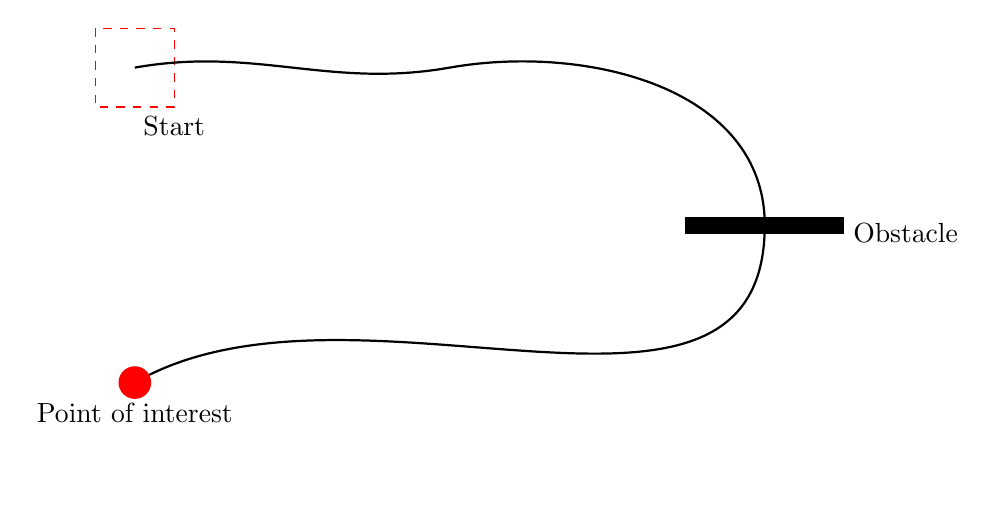
\begin{tikzpicture}
      \draw [red,dashed] (-2.5,2.5) rectangle (-1.5,1.5) node [black,below] {Start}; % Draws a rectangle
      \draw [thick] (-2,2) % Draws a line
      to [out=10,in=190] (2,2)
      to [out=10,in=90] (6,0) 
      to [out=-90,in=30] (-2,-2);    
      \draw [fill] (5,0.1) rectangle (7,-0.1) node [black,right] {Obstacle}; % Draws another rectangle
      \draw [red,fill] (-2,-2) circle [radius=0.2] node [black,below=4] {Point of interest}; % Draws a circle
    \end{tikzpicture}
    \caption{Example graphic made with tikz.}
  \end{center}
\end{figure}
\end{document}